\clearpage

\section{Theorie}
\label{theorie}

\subsection{Mobilfunkstandards}

\subsection{SIM-Karten}

\subsection{Authentifizierungsvorgang}
\label{authentifizierungsvorgang}

\subsection{Milenage Algorithmus}
\label{milenage}
Zwischen \ac{SIM}-Karte und Netzprovider muss eine sichere Authentifizierung und Kommunikation gewährleistet werden können. Dies war wie in Kapitel \ref{geschichte-usim} bereits beschrieben mit dem ersten entwickelten Algorithmus des \ac{3GPP} nicht mehr gewährleistet, weshalb mit der Entwicklung des neuen Netzstandards auch ein neuer Algorithmus entwickelt wurde, namentlich der Milenage Algorithmus. \\
Dieser verfügt über die sieben Funktionen \emph{f1}, \emph{f1*}, \emph{f2}, \emph{f3}, \emph{f4}, \emph{f5}, \emph{f5*} mit Hilfe derer eine sichere Authentifizierung und Schlüsselgenerierung ermöglicht wird. 3GPP hat allerdings wie auch beim Vorgänger diese Funktionen nicht näher spezifiziert und ermöglicht den Netzprovidern eigenen Lösungen zu implementieren. Stattdessen beschrieben sie den Kontext in dem diese Funktionen Anwendung finden und definieren generelle Anforderungen an diese Algorithmen \cite{3gpp.35.205}.

Der Milenage Algorithmus hat wie erwähnt zwei Hauptaufgaben, nämlich einerseits die Authentifizierung, als auch die Generierung eines Schlüssel, um die versendeten Nachrichten zu ver- und entschlüsseln. Wenn es um die Authentifizierung geht muss sich einerseits die SIM-Karte, bzw. das \ac{UE}, gegenüber dem Netzprovider authentifizieren, aber andererseits muss sich auch das Netzwerk gegenüber der SIM-Karte authentifizieren. Damit soll die Möglichkeit der Man-in-the-Middle Attacken reduziert werden, die es einem Außenstehenden erlauben die Kommunikation mitzulesen. Auch so genannte Replay-Attacken, bei denen zuvor aufgezeichnete Daten genutzt werden, sind nicht möglich, auf Grund der \acl{SQN} \cite{spitz11}.

In den nachfolgenden Unterkapiteln wird die Funktionsweise des Algorithmus, sowie die Funktionsweise der eingesetzten Blockschiffrierung \ac{AES} erläutert.

 \subsubsection{Funktionsweise}
 In Kapitel \ref{authentifizierungsvorgang} wurde beschrieben, welche Daten zwischen \ac{AuC} und \ac{UE} verschickt werden, jedoch nicht wie diese Daten generiert werden. Es gibt einige Werte, die auf der \ac{USIM} und der Datenbank des \ac{AuC} fest eingespeichert sind. Diese sind der \ac{OP} und \ac{K}, sowie jeweils fünf Rotations- und XOR-Konstanten (r1, ..., r5 und c1, ... c5). Welche Funktion welche Werte benötigt und generiert zeigt dabei Abbildung \ref{abb:funktionsubersicht}.
 
 \begin{figure}[htp]
  \begin{center}
   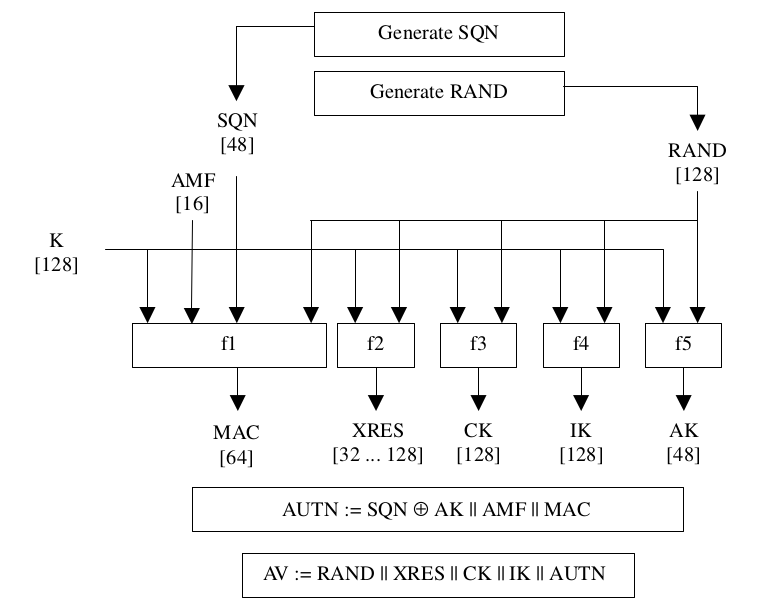
\includegraphics[width=300pt]{generation_of_authentication_vectors}
  \end{center}
  \caption{Übersicht über die Generierung der Authentifizierungsvektoren}
  \label{abb:funktionsubersicht}
 \end{figure}
 
 Die Abbildung \ref{abb:funktionsubersicht} zeigt, dass zu Beginn die \ac{SQN} generiert wird. Diese besteht aus den beiden Teilen SEQ und IND, mit SEQ als der die eigentliche Sequenznummer und IND als Arrayindex. Auf der SIM-Karte sind nämlich die letzten SQNs in einem Array gespeichert. Die empfohlene Größe ist 32, was für IND eine Länge von fünf Bits bedeutet. Mit diesem Index kann nachher die Aktualität der SEQ überprüft werden. Für die Bildung der SEQ selbst gibt es drei verschiedene Möglichkeiten:
 \begin{itemize}
  \item teilweise zeitbasiert
  \item nicht zeitbasiert
  \item komplett zeitbasiert
 \end{itemize}
 
 \subsubsection{AES}

\subsection{PPPoE}

\subsection{raspberry pi}

\subsection{pysim}

\subsection{Die Sprache C}

\subsection{Projektspecs}
